% !TEX root = ../my-thesis.tex
%
\chapter{Material Suplementario del  \autoref{sec:multivar}}\label{sec:appendix:multivar}

{%
\scriptsize
\begin{longtable}{llllllllll}
\caption{Species present in each population.}\label{tab:multivar-s1}\\ 
\toprule
 \textbf{Scientific name}  & \textbf{CAM}  & \textbf{GEN}  & \textbf{MON}  & \textbf{DIL}  & \textbf{DUR}  & \textbf{CAN}  & \textbf{POQ}  & \textbf{TRE}  \endfirsthead 
\hline
\textit{Acer opalus }subsp\textit{. granatense}  & 1 &  & 1 & 1 &  &  &  &  \\
\textit{Adenocarpus decorticans}  & 1 & 1 & 1 & 1 & 1 &  & 1 & 1 \\
\textit{Agrostis canina}  & 1 &  &  &  &  &  &  &  \\
\textit{Andryala integrifolia}  &  &  &  &  &  &  &  & 1 \\
\textit{Arenaria armerina }subsp\textit{. armerina}  & 1 &  &  &  &  &  &  &  \\
\textit{Armeria villosa }subsp\textit{. bernisii}  & 1 &  & 1 &  & 1 &  &  &  \\
\textit{Arrhenatherum elatius }subsp\textit{. bulbosum}  &  &  &  & 1 &  & 1 &  &  \\
\textit{Artemisia absinthium}  &  &  &  &  & 1 &  &  &  \\
\textit{Artemisia barrelieri}  &  &  &  &  & 1 &  &  &  \\
\textit{Artemisia campestris }subsp\textit{. glutinosa}  & 1 & 1 & 1 & 1 & 1 & 1 &  & 1 \\
\textit{Avenula bromoides }subsp\textit{. pauneroi}  &  & 1 & 1 & 1 & 1 &  &  &  \\
\textit{Berberis hispanica}  & 1 &  & 1 & 1 &  &  &  & 1 \\
\textit{Brachypodium retusum}  &  &  &  & 1 &  &  &  & 1 \\
\textit{Carlina corymbosa}  & 1 &  &  &  & 1 &  & 1 & 1 \\
\textit{Carthamus lanatus}  &  & 1 &  &  & 1 & 1 &  & 1 \\
\textit{Celtis australis}  &  &  & 1 &  &  &  &  &  \\
\textit{Centaurea monticola}  &  &  &  &  &  &  & 1 &  \\
\textit{Centaurea ornata}  & 1 &  &  &  &  &  &  &  \\
\textit{Centaurea pulvinata}  &  &  & 1 &  &  &  &  &  \\
\textit{Cerastium gibraltaricum}  & 1 &  & 1 &  & 1 &  &  & 1 \\
\textit{Chondrilla juncea}  & 1 &  &  &  &  &  &  &  \\
\textit{Cirsium odontolepis}  &  &  &  &  & 1 &  &  &  \\
\textit{Cirsium pyrenaicum}  &  &  &  &  &  &  &  & 1 \\
\textit{Clematis vitalba}  &  &  &  & 1 &  &  &  &  \\
\textit{Clinopodium vulgare }subsp\textit{. arundanum}  & 1 &  & 1 &  &  &  &  &  \\
\textit{Corynephorus canescens}  &  &  & 1 & 1 &  &  &  &  \\
\textit{Cotoneaster granatensis}  & 1 &  &  & 1 & 1 &  &  &  \\
\textit{Crataegus granatensis}  & 1 &  &  &  &  &  &  &  \\
\textit{Crataegus monogyna }subsp\textit{. brevispina}  & 1 & 1 & 1 & 1 & 1 &  &  & 1 \\
\textit{Crocus nevadensis}  & 1 &  &  &  &  &  &  &  \\
\textit{Cytisus galianoi}  & 1 &  &  &  &  &  &  &  \\
\textit{Cytisus scoparius }subsp\textit{. reverchonii}  & 1 &  & 1 & 1 & 1 &  &  &  \\
\textit{Dactylis glomerata}  & 1 & 1 &  &  &  &  &  &  \\
\textit{Dactylis glomerata }subsp\textit{. hispanica}  &  &  & 1 & 1 & 1 & 1 &  &  \\
\textit{Daphne gnidium}  &  &  &  &  &  &  &  & 1 \\
\textit{Dianthus pungens }subsp\textit{. brachyanthus}  &  &  & 1 & 1 & 1 &  &  &  \\
\textit{Digitalis purpurea}  &  & 1 &  &  &  &  &  &  \\
\textit{Echinospartum boissieri}  &  &  & 1 &  &  &  &  &  \\
\textit{Elymus hispanicus}  & 1 &  &  &  &  &  &  &  \\
\textit{Erinacea anthyllis}  &  &  &  &  &  &  &  & 1 \\
\textit{Eryngium campestre}  & 1 & 1 & 1 &  &  &  & 1 & 1 \\
\textit{Euphorbia characias}  &  &  &  &  & 1 &  & 1 & 1 \\
\textit{Euphorbia nevadensis}  &  &  &  &  & 1 &  &  &  \\
\textit{Festuca elegans}  & 1 &  & 1 &  &  &  &  & 1 \\
\textit{Festuca hystrix}  &  &  & 1 & 1 &  &  &  &  \\
\textit{Festuca indigesta}  & 1 &  &  & 1 & 1 & 1 &  & 1 \\
\textit{Festuca scariosa}  & 1 & 1 &  &  &  &  &  &  \\
\textit{Fraxinus angustifolia}  &  & 1 &  &  &  &  &  &  \\
\textit{Genista cinerea }subsp\textit{. speciosa}  &  &  & 1 &  &  &  &  &  \\
\textit{Genista versicolor}  & 1 &  &  & 1 & 1 & 1 &  & 1 \\
\textit{Halimium atriplicifolium}  &  &  &  & 1 &  &  &  & 1 \\
\textit{Helianthemum hirtum}  & 1 &  & 1 &  & 1 &  &  &  \\
\textit{Helichrysum italicum }subsp\textit{. serotinum}  &  &  &  &  &  & 1 & 1 & 1 \\
\textit{Helleborus foetidus}  & 1 & 1 & 1 & 1 &  &  &  & 1 \\
\textit{Hieracium pilosella }subsp\textit{. tricholepium}  & 1 &  &  &  &  & 1 &  &  \\
\textit{Hormatophylla spinosa}  & 1 &  &  &  & 1 &  &  &  \\
\textit{Hypericum perforatum}  &  &  & 1 &  & 1 &  & 1 & 1 \\
\textit{Juncus effusus}  &  &  &  &  &  &  & 1 &  \\
\textit{Juniperus communis}  & 1 &  &  &  &  &  &  &  \\
\textit{Juniperus sabina}  & 1 &  &  &  &  &  &  &  \\
\textit{Koeleria vallesiana}  & 1 &  &  & 1 & 1 & 1 & 1 &  \\
\textit{Lathyrus pratensis}  &  &  &  &  & 1 &  &  &  \\
\textit{Lonicera arborea}  & 1 & 1 &  &  & 1 &  &  &  \\
\textit{Marrubium supinum}  & 1 &  &  &  &  &  & 1 & 1 \\
\textit{Ononis aragonensis}  &  &  & 1 & 1 &  &  &  &  \\
\textit{Ononis spinosa}  &  & 1 &  & 1 &  &  & 1 &  \\
\textit{Phlomis crinita}  &  &  &  &  &  &  &  & 1 \\
\textit{Pistacia terebinthus}  &  & 1 &  &  &  &  &  &  \\
\textit{Plantago lanceolata}  &  &  &  &  &  &  &  & 1 \\
\textit{Plantago radicata }subsp\textit{. granatensis}  & 1 &  &  &  &  &  &  &  \\
\textit{Populus nigra}  &  &  &  &  & 1 &  &  &  \\
\textit{Potentilla reuteri}  & 1 &  &  &  & 1 &  &  &  \\
\textit{Prunus avium}  & 1 & 1 &  &  &  &  &  &  \\
\textit{Prunus dulcis}  &  & 1 &  &  &  &  &  &  \\
\textit{Prunus mahaleb}  & 1 &  &  &  &  &  &  &  \\
\textit{Prunus ramburii}  & 1 &  &  &  &  &  &  & 1 \\
\textit{Ptilostemon hispanicus}  &  &  &  &  &  & 1 &  & 1 \\
\textit{Quercus coccifera}  &  & 1 &  &  &  &  &  &  \\
\textit{Quercus faginea}  &  & 1 &  &  &  &  &  &  \\
\textit{Quercus ilex }subsp\textit{. ballota}  & 1 &  & 1 &  & 1 & 1 & 1 & 1 \\
\textit{Quercus pyrenaica}  & 1 & 1 & 1 & 1 & 1 & 1 & 1 & 1 \\
\textit{Retama sphaerocarpa}  &  &  & 1 &  &  &  &  &  \\
\textit{Ridolfia segetum}  &  & 1 &  &  &  &  &  & 1 \\
\textit{Rosa canina}  & 1 & 1 & 1 & 1 & 1 &  & 1 & 1 \\
\textit{Rosa corymbifera}  & 1 &  &  &  &  &  &  &  \\
\textit{Rosa micrantha}  &  &  &  &  &  &  &  & 1 \\
\textit{Rosa pouzinii}  & 1 &  &  &  &  &  &  &  \\
\textit{Rosa sicula}  & 1 &  &  &  &  &  &  &  \\
\textit{Rubus ulmifolius}  & 1 & 1 &  & 1 & 1 &  &  & 1 \\
\textit{Rumex induratus}  &  &  &  & 1 &  &  &  &  \\
\textit{Salix caprea}  &  &  & 1 &  &  &  &  &  \\
\textit{Sanguisorba minor}  & 1 &  &  & 1 &  &  & 1 &  \\
\textit{Santolina rosmarinifolia }subsp\textit{. canescens}  &  &  &  & 1 &  &  &  &  \\
\textit{Santolina rosmarinifolia }subsp\textit{. rosmarinifolia}  & 1 & 1 &  &  &  &  &  &  \\
\textit{Scabiosa turolensis}  & 1 &  &  &  &  &  &  &  \\
\textit{Sedum forsteranum}  & 1 &  &  &  &  &  &  &  \\
\textit{Sedum sediforme}  & 1 &  &  &  &  &  &  & 1 \\
\textit{Silene mellifera}  &  &  & 1 & 1 &  &  & 1 &  \\
\textit{Smilax aspera}  &  & 1 &  &  &  &  &  &  \\
\textit{Solidago virgaurea}  &  &  & 1 &  &  &  &  &  \\
\textit{Sorbus aria}  & 1 &  & 1 &  &  &  &  &  \\
\textit{Teucrium capitatum}  &  &  & 1 &  &  &  &  &  \\
\textit{Teucrium similatum}  & 1 &  &  &  &  &  &  &  \\
\textit{Thymus mastichina}  & 1 &  &  & 1 &  & 1 &  & 1 \\
\textit{Thymus serpylloides }subsp\textit{. serpylloides}  &  &  &  &  &  & 1 &  & 1 \\
\textit{Thymus zygis}  &  &  &  &  &  &  & 1 & 1 \\
\textit{Vicia sp.}  &  & 1 & 1 &  & 1 &  &  &  \\
\textit{Vinca difformis}  &  &  &  & 1 &  &  &  &  \\ 
\hline
\textbf{Total}  & 54 & 25 & 34 & 31 & 32 & 14 & 17 & 36 \\
\bottomrule
\end{longtable}

}%

\newpage


\chapter{Material Suplementario del  \autoref{sec:dendro}}\label{sec:appendix:dendro}

\begin{figure}
\centering
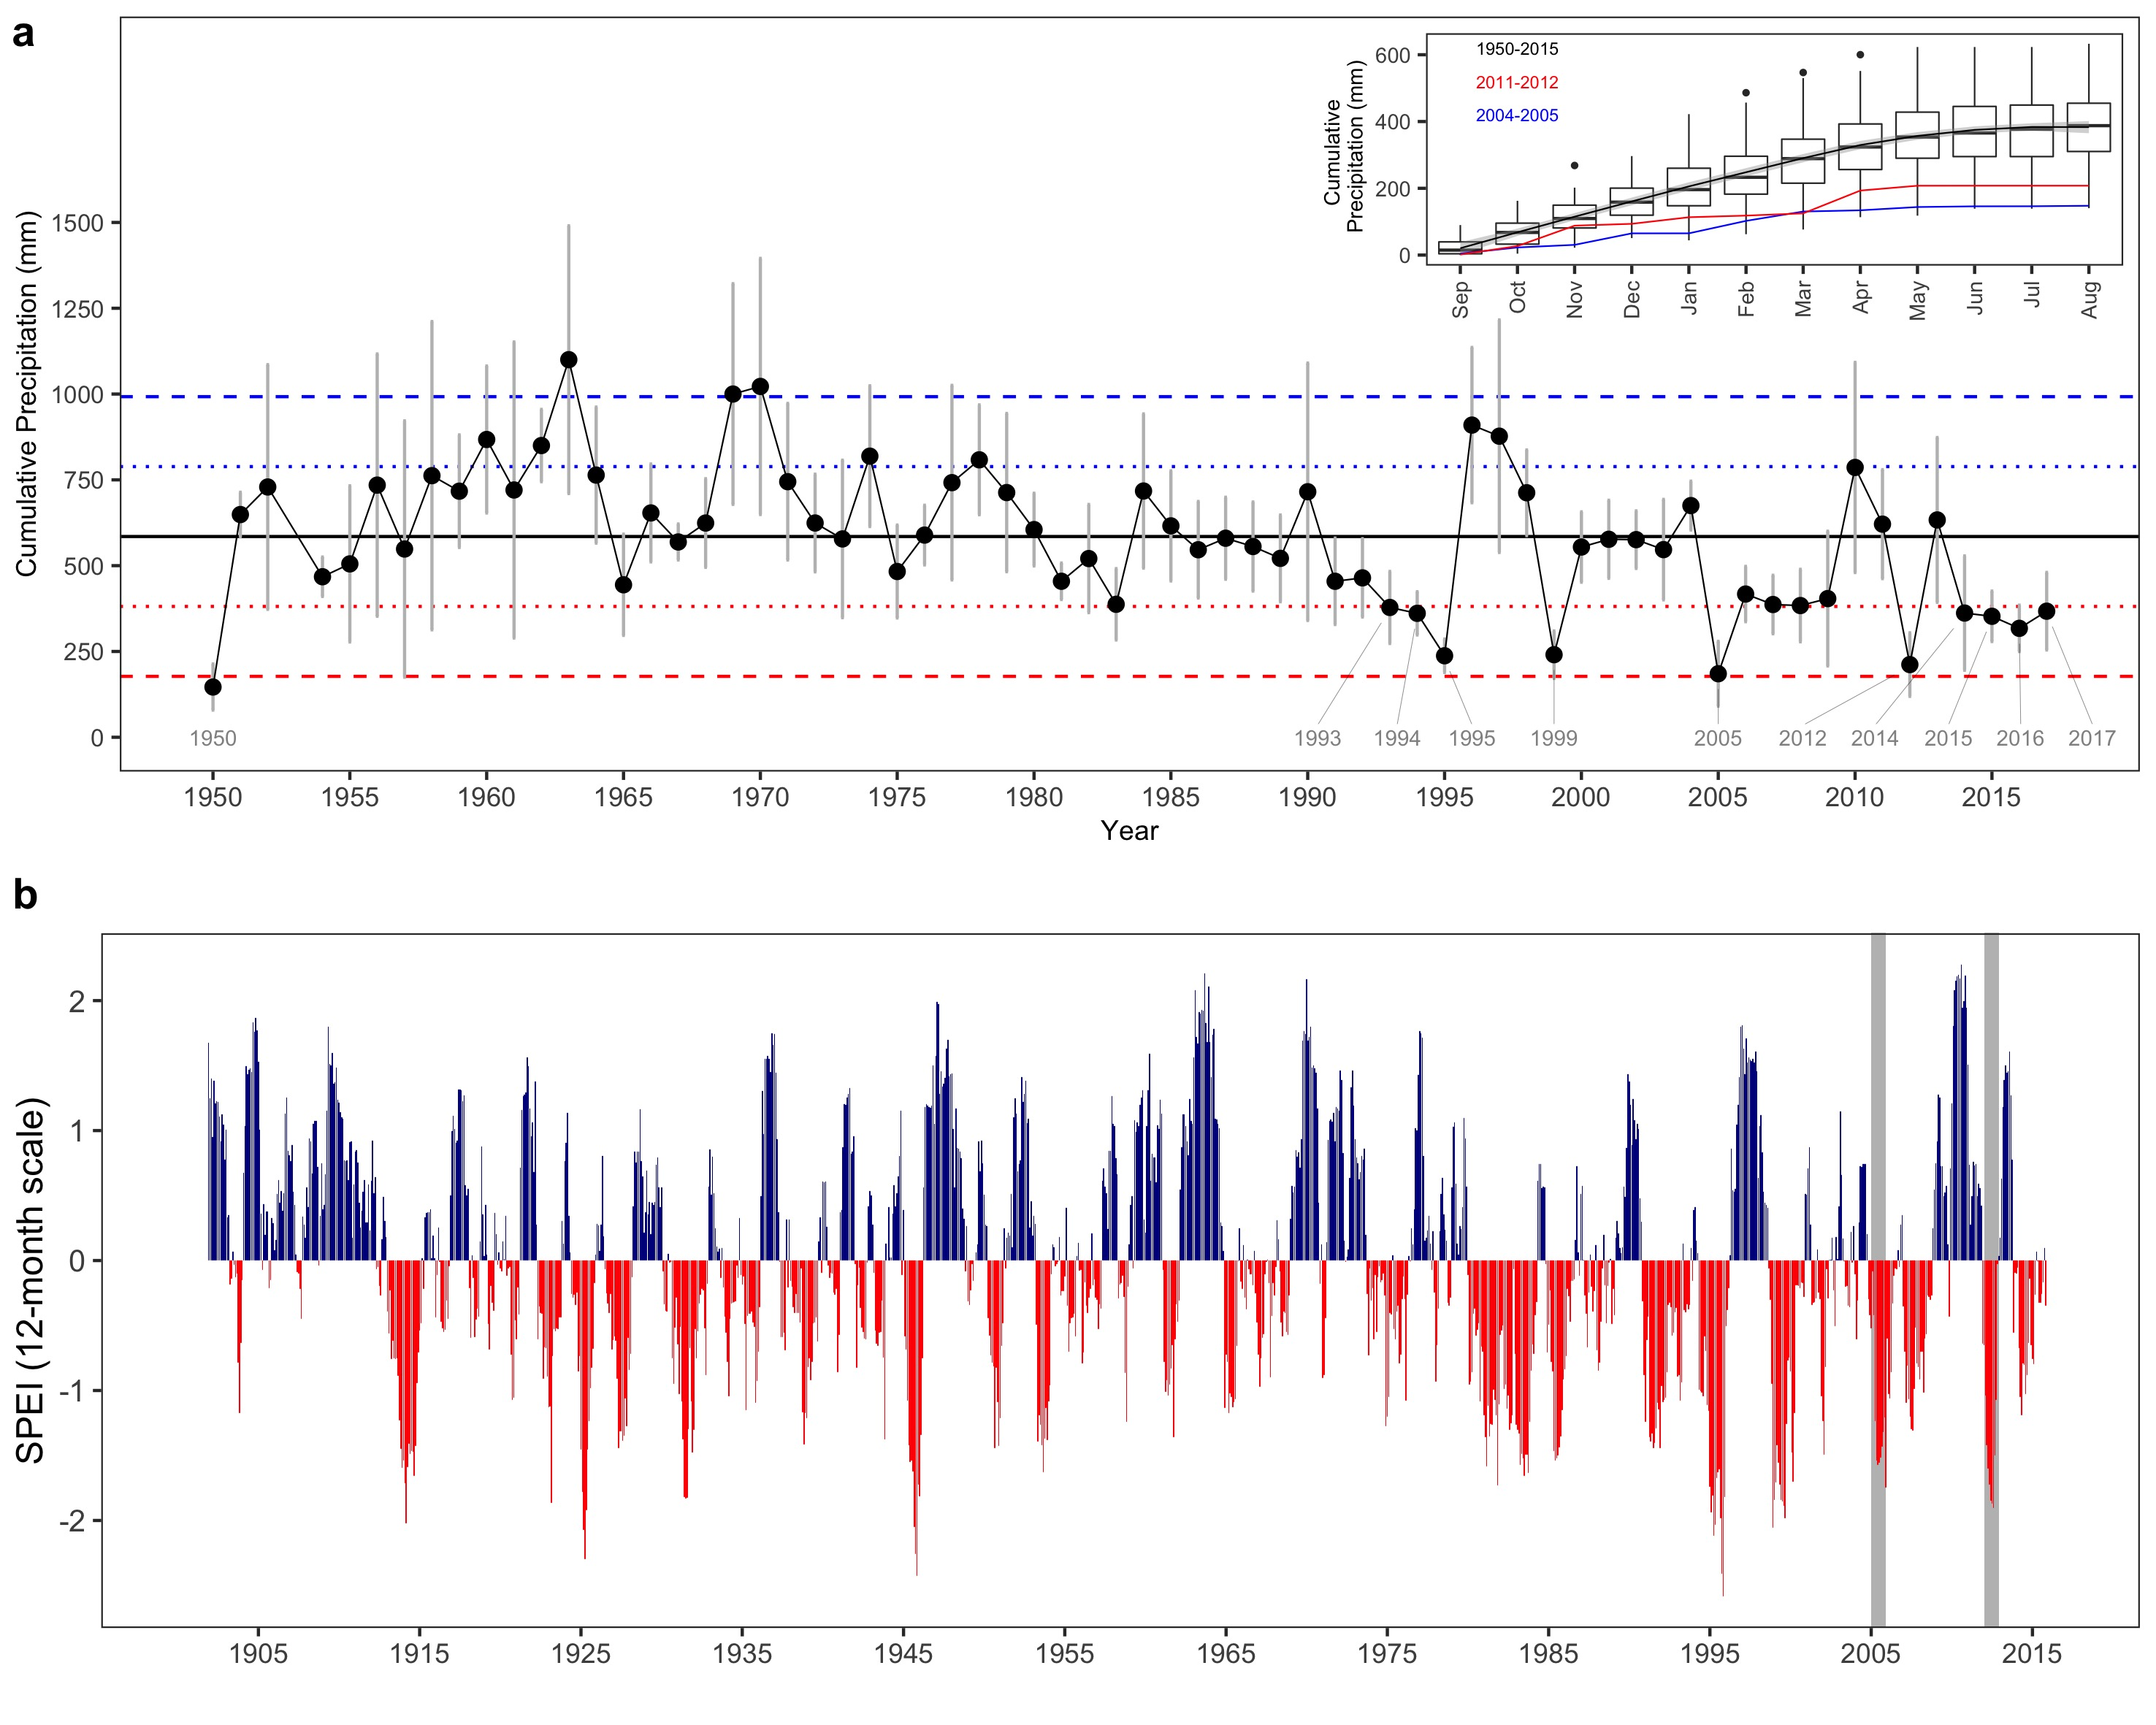
\includegraphics[width=\textwidth]{img/dendro/dendro-s1climate} 
\caption{\textbf{a)} Temporal evolution of cumulative precipitation (hydrological year) during the period 1950-2017. Points represent the mean, and error bars the standard error. The black line indicates mean for the entire period (585 mm). The red lines represent -1 and -2 standard deviation (dotted and dashed lines, respectively). The blue lines represent +1 and +2 standard deviation (dotted and dashed lines, respectively). Years with average values below -1SD are labeled. Data from 28 meteorological stations distributed around the Sierra Nevada area (from the National Spanish Meteorological Services, AEMET). Inset plot: cumulative precipitation during the hydrological years 2004-2005 (blue line) and 2011-2012 (red line). The boxplot representing the average from 1950-2015 period. Data from meteorological station Granada, Base Aérea. \textbf{b)} Drought severity in Sierra Nevada for the 1901-2016 period based on the Standardized Precipitation-Evapotranspiration Index (SPEI). Data from Global SPEI database (http://spei.csic.es/database.html). We took the SPEI data for a 12-month scale and for all 0.5\textdegree grid cells covering Sierra Nevada. Horizontal gray bars indicate the years 2005 and 2012.}  
\label{fig:dendro:s1-climate}
\end{figure}

\newpage
\begin{figure}
\centering
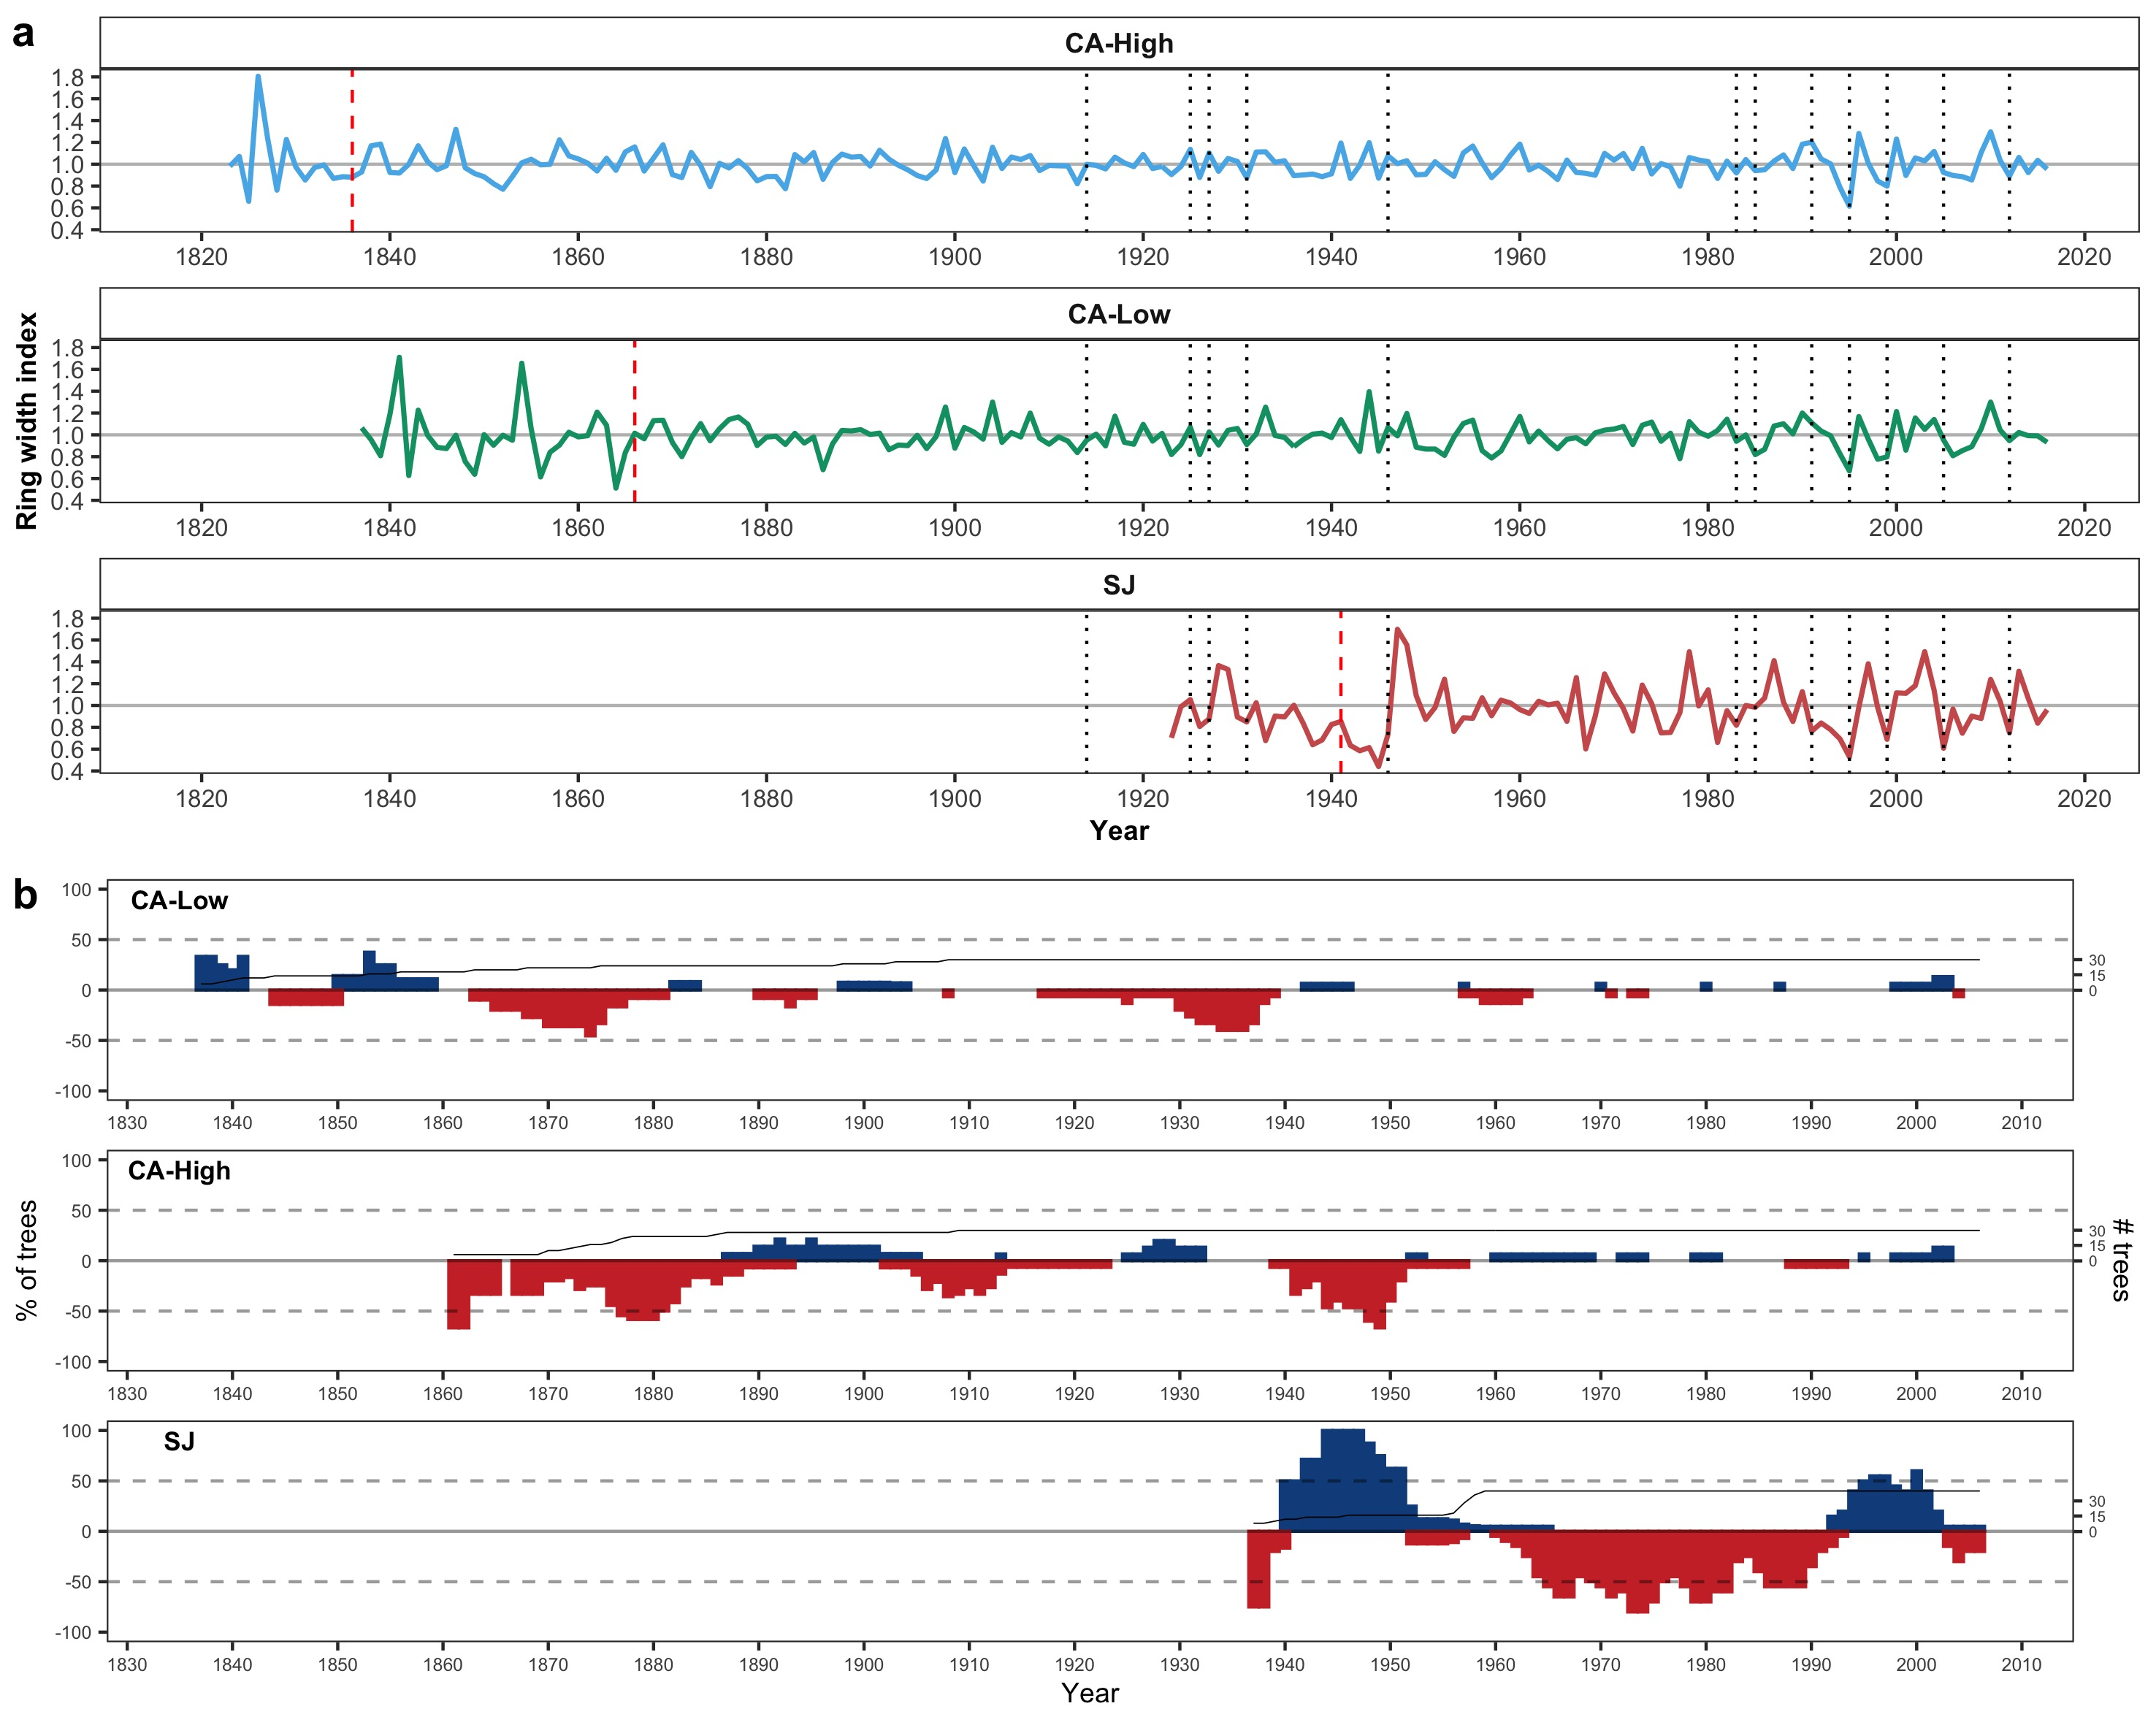
\includegraphics[height=14 cm]{img/dendro/dendro-s2chronos} 
\caption{\textbf{a)} Residual tree-ring chronologies determined for the \Qp sites. Dashed red lines indicate the start of the reliable period (EPS > 0.85). Dotted black lines show the severe drought years identified in our climatic data (Table S3 and Figure S1). b) Percentage of \Qp trees affected by GC > 50 \% by site. Black line shows number of trees (right-axis). Data for number of trees > 2 is shown.
}  
\label{fig:dendro:s2chronos}
\end{figure}
